\documentclass[11pt,a4paper]{article}

\usepackage[T1]{fontenc}
\usepackage[utf8]{inputenc}
\usepackage{lmodern}
\usepackage[margin=2.4cm]{geometry}
\usepackage{microtype}
\usepackage{graphicx}
\usepackage{xcolor}
\definecolor{keptc}{HTML}{23324A}   % effect that survives the composition adjustment
\definecolor{mixc}{HTML}{9AA1A9}    % a bar whose direction contradicts discovery
\definecolor{emptyc}{HTML}{E8EBEE}  % the unfilled remainder of a bar

\usepackage{booktabs}
\usepackage{longtable}
\usepackage{array}
\usepackage{pdflscape}
\usepackage{amsmath}
\usepackage{amssymb}   % \mathbb for the matrix spaces in the Boruta section
\usepackage[font=small,labelfont=bf]{caption}
% let figures share a page with text instead of floating onto pages of their own
\renewcommand{\topfraction}{0.9}
\renewcommand{\bottomfraction}{0.8}
\renewcommand{\textfraction}{0.07}
\renewcommand{\floatpagefraction}{0.75}
\setcounter{topnumber}{2}
\setcounter{totalnumber}{3}
\usepackage{authblk}
\usepackage[backend=bibtex,bibstyle=numeric,citestyle=authoryear,natbib=true,
            maxcitenames=1,mincitenames=1,giveninits=true,sorting=none,doi=true,url=false,isbn=false]{biblatex}
\usepackage[colorlinks=true,citecolor=blue,linkcolor=blue,urlcolor=blue,filecolor=blue]{hyperref}
\usepackage{xurl}
\addbibresource{references.bib}

\title{Boruta-Driven Explainable Machine Learning for Identifying Gene Signatures in Laser-Captured
Dopamine Neurons of Parkinson's Disease}
\author{Ali Sareminia}
\date{}

\begin{document}
\maketitle

\begin{abstract}
\noindent\textbf{Background.} Expression studies of the substantia nigra in Parkinson's disease (PD) are
confounded by the loss of the very cells they measure. Laser-capture microdissection (LCM)
isolates dopamine neurons before sequencing, but each LCM study is small, and a panel
selected in one is rarely tested anywhere else.

\noindent\textbf{Methods.} Four LCM datasets were merged at one profile per person (63 donors, 30 control, 33
PD; 5,622 genes measured and expressed in all four). A Random Forest on within-person gene ranks was
evaluated by repeated cross-validation, leave-one-study-out and label permutation, and Boruta selected a
30-gene panel. Both models were then frozen and applied without refitting to eight public bulk nigra cohorts
(158 donors, 72 control, 86 PD, after 14 shared brains were removed). We scored each donor's dopamine-neuron content, estimated
the CALB1-versus-SOX6 subtype mix from published single-nucleus markers, and repeated the whole
analysis with that mix regressed out of every gene.

\noindent\textbf{Results.} Nine of the 30 panel genes replicated in the independent bulk donors with the same
direction of effect and a Benjamini--Hochberg $q<0.05$ before any adjustment for neuron content (\textit{RBM4B}, \textit{USP12}, \textit{SOX6},
\textit{ADGRB3}, \textit{SH3GL3}, \textit{DNAJB1}, \textit{CNTN4}, \textit{ZMYND8} and \textit{SSTR1}), and
once each donor's dopamine-neuron content was removed from every gene 23 of the 30 effects still agreed in
sign with the laser-captured neurons ($P=0.003$). The classifier that selected them reached an area under the
ROC curve (AUC) of 0.73 (SD 0.03) across
donors and 0.68 with a whole study held out (label shuffles $P=0.005$). In bulk tissue the frozen classifier
pooled 0.70 (95\% CI 0.62--0.78) and the panel forest 0.84 (0.77--0.90), but eight dopamine-neuron markers
alone reached 0.86. Removing neuron content left the panel at 0.76 and the classifier at 0.62. Genes lower in
PD are markers of SOX6 dopamine neurons and genes higher are markers of CALB1 neurons ($P=0.0012$; $P=0.004$
against gene sets matched on effect size), the split that single-nucleus work reports for selective
vulnerability. Over-representation analysis against the measured background returned four
synapse and calcium-binding terms. When each donor's estimated subtype mix was regressed out of every gene,
out-of-fold AUC fell from 0.76 to 0.67 ($P=0.009$) yet stayed above chance, and 23 of 30 genes kept at least
half of their effect.

\noindent\textbf{Conclusions.} The panel is a reproducible set of candidate genes rather than a diagnostic
score: nine of its members survive a test in independent tissue, while most of what the classifier itself uses
is a shift in which dopamine neurons remain rather than a change inside surviving neurons. Reports of nigral expression signatures in PD
should state how much survives an explicit composition adjustment.

\medskip
\noindent\textbf{Keywords:} Parkinson's disease; substantia nigra; laser-capture microdissection; external
validation; cell composition; Boruta; SHAP; dopamine-neuron subtypes
\end{abstract}

\section{Introduction}

Parkinson's disease is the fastest-growing neurological cause of disability worldwide \citep{gbd2024}, and its
prevalence keeps rising as populations age \citep{benshlomo2024,bloem2021}. The motor syndrome follows the
loss of neuromelanin-containing dopamine neurons of the substantia nigra pars compacta \citep{kordower2013}.
Why those neurons go first is still argued over, with $\alpha$-synuclein aggregation, mitochondrial and
lysosomal failure and the metabolic cost of pacemaking all proposed \citep{morris2024,surmeier2017}.
Single-nucleus sequencing sharpened the question by showing that vulnerability differs between dopamine
neuron subtypes: the SOX6\_AGTR1 population is depleted in PD while several CALB1 populations are relatively
spared \citep{kamath2022}. Molecular taxonomies of midbrain dopamine neurons agree on that broad
SOX6--CALB1 division \citep{poulin2020}.

This is a problem for expression studies of nigral tissue. When neurons die the tissue that remains contains
proportionally more glia, and in PD brain much of what looked like disease biology turns out to be a change in
cell composition \citep{nido2020}. Laser-capture microdissection removes part of the problem by collecting the
neurons themselves before sequencing \citep{nichterwitz2016}, and several LCM datasets of human nigral
dopamine neurons are public \citep{zheng2010,tiklova2021,zaccaria2022}. None of them holds more than 22
people.

Small cohorts and tens of thousands of genes are an easy way to overfit. Selecting genes on all samples before
cross-validation biases the error estimate \citep{ambroise2002}, as does tuning a model on the data used to
score it \citep{varma2006}; both remain common in genomics and in machine-learning-based science more broadly
\citep{whalen2022,kapoor2023}. Repeated measurements from one donor are not independent \citep{hurlbert1984,
lazic2010}, and treating pools or cells as the unit of analysis inflates false discoveries in transcriptomics
\citep{squair2021,zimmerman2021}. The most informative test holds out whole studies \citep{bernau2014},
because platform and batch effects can exceed the biology \citep{leek2010}.

In earlier work we merged four LCM cohorts at one row per person and used Boruta \citep{kursa2010,breiman2001}
with SHAP \citep{lundberg2020} to select and explain a gene panel. Two questions were left open. First,
whether the panel carries across to data the model has never seen, which for nigral expression means bulk
tissue, where most public cohorts live. Second, whether what the panel measures is a change inside dopamine
neurons or a change in which dopamine neurons are left to measure. Here we fix both models before touching any
external data, test them in eight public bulk cohorts after removing brains shared with the discovery studies,
and then ask how much of the signal survives an explicit adjustment for each donor's estimated dopamine-neuron
subtype mix.

\section{Methods}

\subsection{Discovery cohort}

All expression data came from the Gene Expression Omnibus \citep{barrett2013}. Four LCM studies of nigral
dopamine neurons were merged at one profile per person (Table~\ref{tab:cohort}): GSE182622, RNA sequencing of
pools of neuromelanin-positive neurons \citep{tiklova2021}; GSE20141 and GSE24378, Affymetrix HG-U133 Plus 2.0
and HG-U133 X3P profiles \citep{zheng2010}; and GSE169755, RNA sequencing of two libraries per brain
\citep{zaccaria2022}. Replicate pools and libraries from one donor were averaged, so that 192 pools became 22
donors in GSE182622 and 12 libraries became 6 brains in GSE169755. Of 28,180 genes, 10,164 were measured on
all four platforms and 5,622 were expressed in every study. Each study was standardised on its own without
reference to diagnosis. A classifier trained to name each donor's study placed every donor correctly before
that step and 1\% afterwards, against a 25\% chance rate (Fig.~\ref{fig:design}).

\begin{figure}[htbp]\centering

\includegraphics[width=\textwidth]{figures/Figure01_study_design.pdf}
\caption{Study design. (a) Nigral dopamine neurons were isolated by laser-capture microdissection in each
study. (b) Four cohorts, 63 people, one profile per person after replicate pools and libraries were averaged.
(c) Harmonisation: 28,180 genes reduce to 5,622 measured and expressed in every study, and standardising
within study removes study identity, which a classifier could otherwise recover perfectly. (d) The analysis in
five stages, with the figure each one produces.}
\label{fig:design}
\end{figure}

\input{table_cohorts}

\subsection{The core classifier}

Three steps make up the model, and each answers a specific problem with merging studies. First, genes are
ranked within each person, so a profile enters the model as the order of its genes rather than as
platform-dependent intensities; a rank transform of this kind is the usual defence when arrays and sequencing
are combined \citep{leek2010}. Second, the 5,622 ranks are reduced to 30 principal components fitted on the
training donors only, which keeps the dimensionality below the sample size and keeps test donors out of the
projection \citep{ambroise2002}. Third, a Random Forest \citep{breiman2001} is fitted on those components with
1,000 trees, \texttt{max\_features} 0.5, one sample per leaf and balanced class weights, using scikit-learn
\citep{pedregosa2011}. A forest suits this setting because it assumes no distribution, tolerates correlated
predictors, and reports an out-of-bag error from the samples each tree did not see \citep{breiman2001}. Performance was estimated by
five repeats of five-fold cross-validation split by person (seeds 1000--1004), by leave-one-study-out, and
against 200 permutations of the diagnosis labels within each study. The model configuration was chosen inside
the folds among 97 Random Forest variants, so that the reported estimate is not the maximum over the
comparison \citep{varma2006}.

\subsection{The 30-gene panel}

Boruta is the selection step this paper depends on, so we state it as the test it is \citep{kursa2010}. Let
$X \in \mathbb{R}^{n \times p}$ hold the $p = 5{,}622$ genes of $n = 63$ donors and let $y$ be the diagnosis.
At iteration $t$ every column is copied and shuffled,
%
\begin{equation}
\tilde{X}^{(t)}_{\cdot j} = X_{\pi^{(t)}_j(\cdot),\, j}, \qquad \pi^{(t)}_j \sim \text{Unif}(S_n),
\end{equation}
%
which destroys any relation to $y$ while keeping each gene's own distribution; these are the shadow features.
A Random Forest is fitted to $[X, \tilde{X}^{(t)}]$ and gives importances $Z^{(t)}_j$. A gene scores a hit
when it beats the shadow columns of that same run,
%
\begin{equation}
h^{(t)}_j = \mathbf{1}\!\left\{ Z^{(t)}_j > Q_{0.99}\!\left( Z^{(t)}_{\tilde{1}}, \dots, Z^{(t)}_{\tilde{p}} \right) \right\},
\qquad
H_j = \sum_{t=1}^{T} h^{(t)}_j ,
\end{equation}
%
and under the null that the gene carries nothing, $H_j \sim \text{Binomial}(T, \tfrac{1}{2})$. Genes are
confirmed or rejected by a two-sided binomial test on $H_j$ with a Bonferroni correction over the $p$ genes;
rejected genes are dropped from later iterations, and whatever is still undecided when $t$ reaches $T$ stays
tentative. Using $Q_{0.99}$ of the shadow importances instead of their maximum is the stricter variant, which
suits a 63-donor cohort.

Boruta is all-relevant rather than minimal-optimal: it keeps every gene that carries signal instead of the
smallest set that predicts, which is what one wants when the aim is interpretation
\citep{kursa2010,degenhardt2019}. We used $T = 100$ iterations and a 500-tree forest, run on all 63 donors and
again inside every training fold, so Table~\ref{tab:genes} reports how often each gene is reselected rather
than assuming the selection is stable \citep{degenhardt2019}. The panel holds 30 genes, 18 higher and 12 lower
in PD.

TreeSHAP values \citep{lundberg2020} were computed out of fold. Differential expression used
the two-sided Wilcoxon rank-sum test \citep{mannwhitney1947} with Benjamini-Hochberg control \citep{bh1995}, and
per-study effects were combined as Hedges' $g$ \citep{hedges1981} in a random-effects meta-analysis
\citep{dersimonian1986}.

\subsection{Model locking and external cohorts}

Both models, the core classifier and a forest restricted to the 30 panel genes, were fitted on all 63
discovery donors and stored before any external cohort was downloaded. Nothing was refitted, re-selected or
re-tuned afterwards. Eight public bulk substantia nigra cohorts were then scored: GSE7621
\citep{lesnick2007}, GSE8397 \citep{moran2006}, GSE20163 and GSE20164 \citep{zheng2010}, GSE20292
\citep{zhang2005}, GSE49036 \citep{dijkstra2015}, GSE114517 \citep{simchovitz2020} and GSE168496
\citep{tranchevent2023}. Probe sets were mapped to gene symbols through the g:Profiler conversion service
\citep{kolberg2023}; HG-U133A arrays were mapped through the Plus 2.0 namespace, which recovers 4,584 of the
5,622 discovery genes. Each cohort was standardised within itself and then ranked within each person, exactly
as in discovery. Four panel genes are absent from that older array design: \textit{SOX6}, \textit{CNTN4},
\textit{ELOVL7} and \textit{C11orf54} are not represented on HG-U133A, so GSE8397, GSE20163, GSE20164 and
GSE20292 contribute 26 of the 30 panel genes and the per-gene meta-analysis of those four rests on the other
four cohorts. Rather than drop those cohorts or refit the frozen models, a missing gene was given the cohort
mean, that is a standardised value of zero, so that it moves no donor's score in either direction; the
external estimates for the four genes therefore come only from the cohorts that measure them.

Donor identifiers were compared with the discovery studies. GSE20292 shares 12 brains with GSE20141 and
GSE20163 shares 2, identified by matching donor numbers; those donors were removed, leaving 158 people (72
control, 86 PD). Because shared brain banks can leak in ways identifiers do not show, every cohort was also
scored by strictly independent models retrained without any discovery study from the same bank. Significance
came from 10,000 permutations of diagnosis within cohorts; confidence intervals from 4,000 donor bootstraps
\citep{efron1979}. Cohort AUCs were pooled with weights equal to the number of PD--control pairs, and ROC
curves were averaged vertically with the same weights so that the drawn curve has the pooled area
\citep{hanley1982}.

The dependence of the external result on the less stable members of the panel was measured by repeating the
whole frozen-panel procedure with the panel restricted by fold frequency, at every threshold from 0 to 100\%
in steps of 4\%, and by comparing each panel with 200 random panels of the same size drawn from the 5,622
measured genes and put through the identical steps. Fold frequencies come from the discovery donors alone and
were fixed when the panel was selected.

Each panel gene was also tested on its own in the external donors. Cohort-level standardised effects were
combined by inverse-variance meta-analysis, tested two-sided against the standard normal and corrected by the
Benjamini--Hochberg procedure over the 30 genes of the panel, before and after the neuron-content adjustment
described next. Agreement of sign with the discovery effect was tested by a two-sided binomial test against
one half.

\subsection{Dopamine-neuron content and subtype mix}

Two adjustments were made, and they answer different questions. The first asks whether a score merely tracks
how much dopamine-neuron material a bulk sample contains: eight canonical dopamine-neuron markers
(\textit{TH}, \textit{SLC6A3}, \textit{SLC18A2}, \textit{DDC}, \textit{KCNJ6}, \textit{ALDH1A1},
\textit{NR4A2} and \textit{EN1}) were standardised within each cohort and averaged into a
neuron score, and each model score was residualised on it within each cohort. All eight are measured in every
external cohort. The second asks which dopamine
neurons remain. Marker $z$ scores for every dopamine-neuron subtype were taken from Supplementary Table 8 of
\citet{kamath2022}; a lineage score was defined for each gene as its mean marker strength over the six CALB1
subtypes minus its mean over the four SOX6 subtypes. The 50 strongest markers on each side, with panel genes
excluded, gave a per-donor composition score, standardised within study. That score was then regressed out of
every one of the 5,622 genes, and the whole discovery pipeline was run again on the adjusted data with the
same folds and the same model. Sensitivity runs used 25, 100 and 200 markers, SOX6\_AGTR1 markers alone, and
composition together with overall dopamine purity.

Because that neuron score is our own construction, it was checked against reference-based deconvolution.
The reference is the single-nucleus midbrain atlas of \citet{smajic2022} (GSE157783): 41,434 nuclei from six
controls and five people with Parkinson's disease, carrying the authors' own cell-type labels. Each cell type
was summarised once per reference donor as counts per million, the per-donor profiles were averaged, and a
signature matrix of 1,626 genes was built by keeping, for each cell type, the genes with the largest fold
change over the remaining types (condition number 24.0). Every external donor was then deconvolved three
ways: non-negative least squares; $\nu$ support-vector regression, the estimator behind CIBERSORT
\citep{newman2015}; and non-negative least squares weighted by the inverse across-donor variance of each
gene, the idea behind MuSiC \citep{wang2019}. Between 799 and 1,567 signature genes were measured per cohort.
The deconvolved dopamine-neuron proportion was compared with the eight-marker score, and the external scores
were residualised on it in place of that score. This analysis uses all 173 external donors, without the
donor-overlap removal, so its absolute AUCs sit below those of Table~\ref{tab:external}; the three
adjustments are computed on the same donors and are therefore comparable with each other.

\subsection{Pathway analysis}

Over-representation was tested with g:GOSt \citep{kolberg2023} using the 5,622 measured genes as the
background and Benjamini-Hochberg correction across all 3,547 terms \citep{bh1995}, against GO, Reactome
\citep{milacic2024}, KEGG \citep{kanehisa2023} and WikiPathways \citep{agrawal2024}. Because a gene list of
this size can return terms by chance, the same settings were applied to 100 random gene lists of each size
drawn from the same background, and to lists matched on differential-expression rank; the calibrated $P$ value
is the share of those lists reaching a smaller adjusted $P$ than the panel. A ranking-based analysis was also
run for completeness: gene set enrichment analysis \citep{subramanian2005} over all 5,622 genes against 1,967
sets from Hallmark \citep{liberzon2015}, Reactome, KEGG and GO, with the null built by shuffling donor
diagnoses within study rather than genes, and single-sample scores per donor \citep{barbie2009}. Gene set
definitions came from Enrichr's libraries \citep{kuleshov2016}.

\subsection{Gene-level annotation}

Table~\ref{tab:genes} collects what is known about each panel gene, and every cell in it is either measured
here or taken from a named public resource at a stated release. Protein names and functions are from UniProt
\citep{uniprot2025}, with the accession given so each statement can be checked. Association scores with
Parkinson disease, the tractability evidence and the count of drug or clinical candidates are from the Open
Targets Platform \citep{buniello2025}. Dopamine-neuron subtype identity is the lineage score described above
\citep{kamath2022}.

Published links to the disease were found with one protocol applied to every gene, so that the absence of a
link is as checkable as its presence. We searched Europe PMC \citep{europepmc2024} for the gene symbol, its
approved name and every HGNC alias, in the title or abstract, together with Parkinson, parkinsonism, Lewy,
synuclein, LRRK2, PINK1, parkin, glucocerebrosidase, dopaminergic neuron, substantia nigra, MPTP, rotenone,
6-hydroxydopamine or paraquat; for open-access papers we also read the full text sentence by sentence. A
paper was kept only when one sentence reports a finding about the gene itself in that setting. Reviews,
acronym collisions (\textit{FUS} returns focused ultrasound, \textit{SCAI} a cardiology society) and
retracted papers were excluded, and every citation was checked against Crossref for retractions and
corrections. The complete search, with each hit and its disposition, is Supplementary Table~S1.

\subsection{Reproducibility}

Every analysis ran in public Kaggle notebooks, each writing the tables the figures read; no figure recomputes
a result. Random seeds are fixed and reported in the notebooks.

\section{Results}

\subsection{One profile per person, and a classifier that works at donor level}

The merged cohort holds 63 people from four studies (Table~\ref{tab:cohort}), one profile each, on 5,622
genes. Standardising within study removed study identity almost completely (Fig.~\ref{fig:design}c).

On these donors the classifier reached an AUC of 0.725 (SD 0.032) and an accuracy of 0.692 across 25
person-level folds, with sensitivity 0.56 and specificity 0.83 (Fig.~\ref{fig:performance}). Holding out a
whole study gave 0.678, ranging from 1.00 in the six-brain GSE169755 to 0.55 in GSE20141. Against 200 label
permutations the observed AUC of 0.707 sat above a null centred on 0.498 ($P=0.005$), and choosing the model
inside the folds rather than once on all data gave 0.741, so the estimate is not an artefact of the comparison
\citep{varma2006}. A forest on all 5,622 genes without the rank and component steps reached 0.66.

\begin{figure}[htbp]\centering
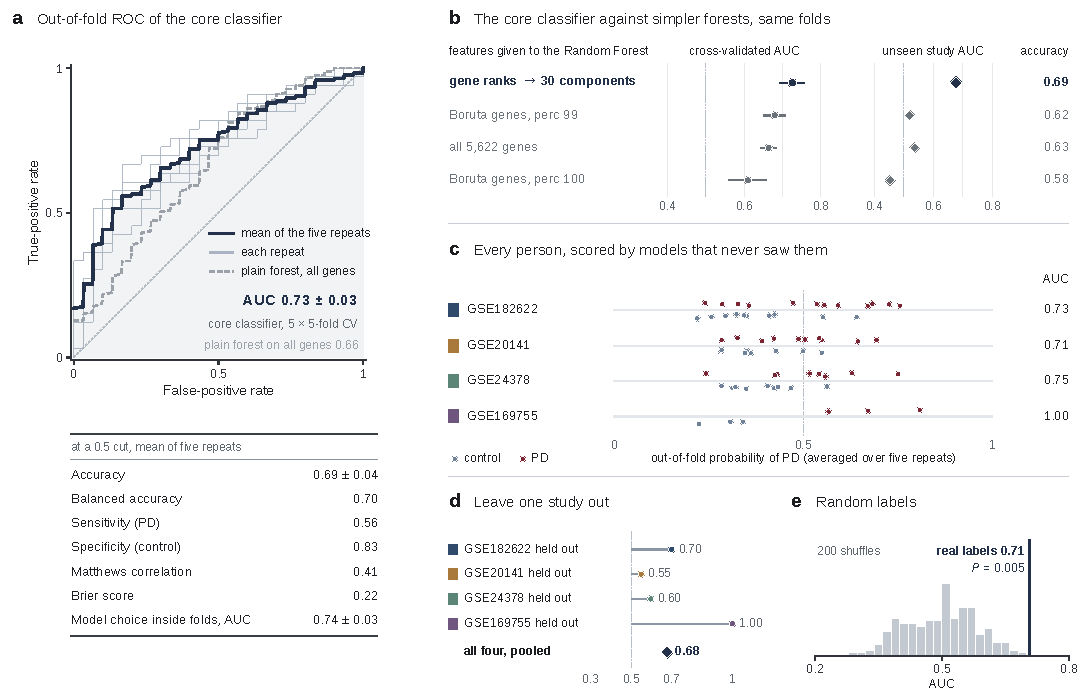
\includegraphics[width=\textwidth]{figures/Figure02_classifier_performance.pdf}
\caption{The core classifier. (a) Out-of-fold ROC over 25 person-level folds. (b) The same folds for simpler
forests. (c) Every donor's out-of-fold score. (d) Leave-one-study-out. (e) 200 permutations of the diagnosis
labels within study.}
\label{fig:performance}
\end{figure}

\subsection{What the model uses}

Boruta confirmed 30 genes, 18 higher and 12 lower in PD. \textit{RBM4B}, \textit{PLXNC1} and \textit{GPNMB}
lead the SHAP ranking and were kept in 100\%, 96\% and 92\% of training folds; single genes reach AUCs of
0.63--0.78 on their own (Fig.~\ref{fig:shaprank}, Fig.~\ref{fig:beeswarm}).

\begin{figure}[htbp]\centering
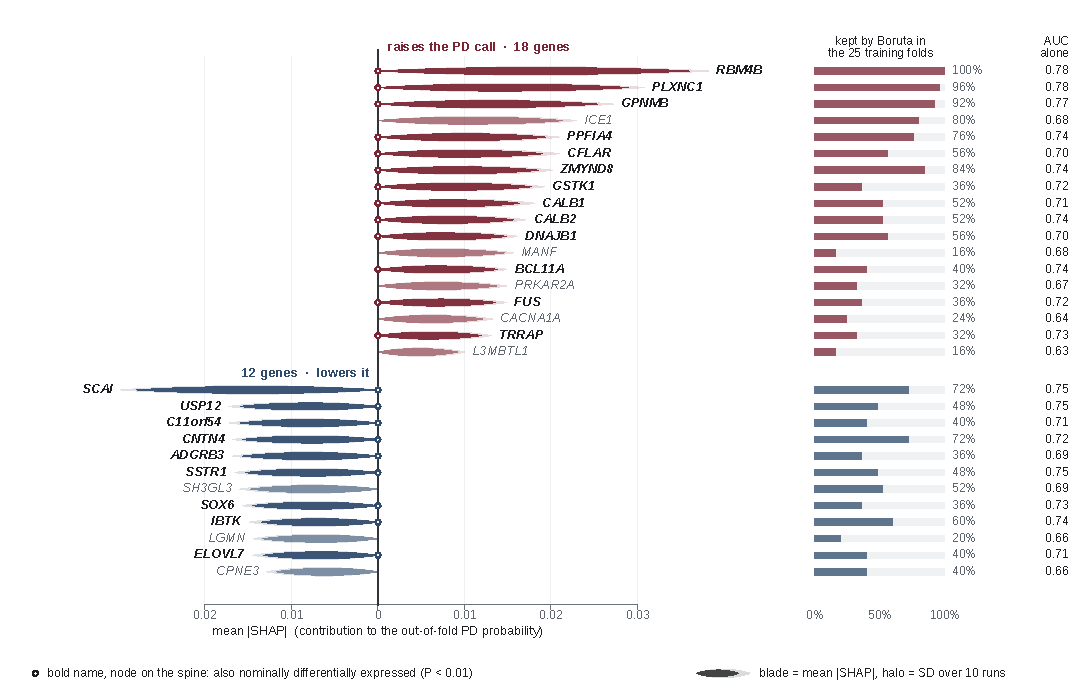
\includegraphics[width=\textwidth]{figures/Figure03_shap_ranking.pdf}
\caption{The 30 Boruta genes ranked by mean absolute SHAP contribution to the out-of-fold PD probability,
split by direction, with the share of training folds that reselected each gene and the AUC of each gene alone.
Bold names are also nominally differentially expressed.}
\label{fig:shaprank}
\end{figure}

\begin{figure}[htbp]\centering
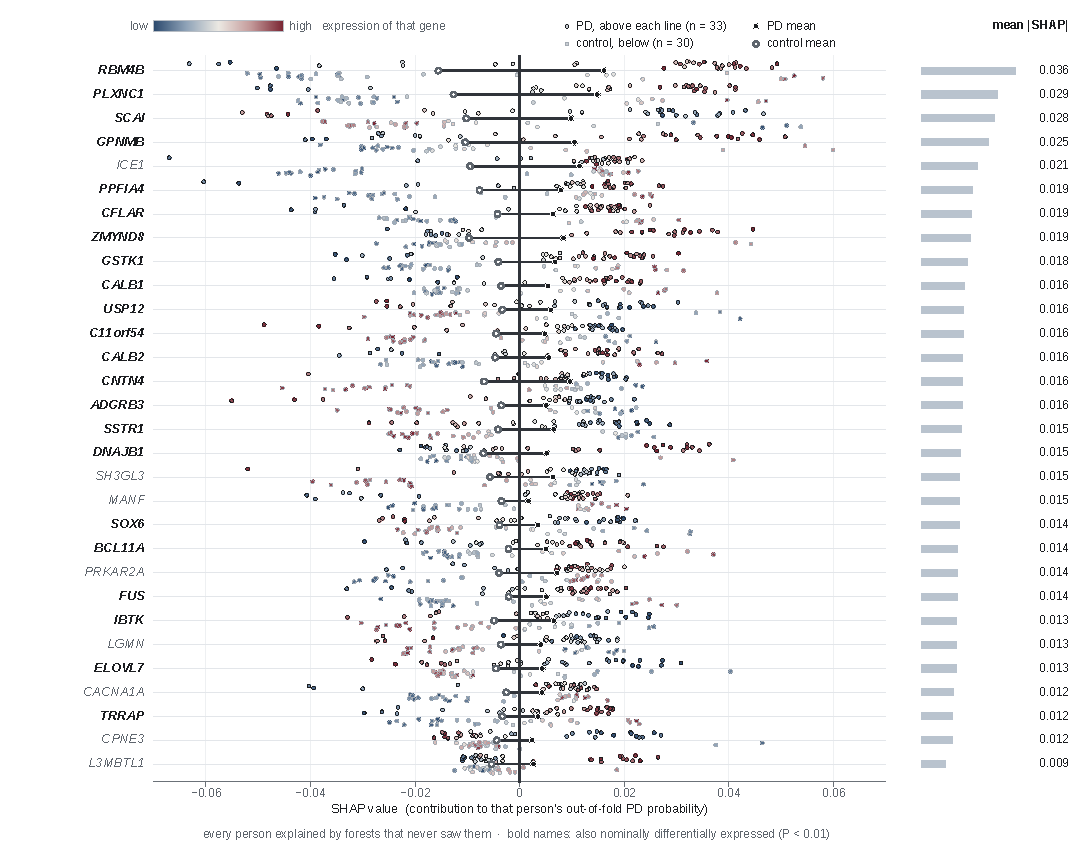
\includegraphics[width=\textwidth]{figures/Figure04_shap_beeswarm.pdf}
\caption{SHAP values of every donor for every panel gene, coloured by that donor's expression rank.}
\label{fig:beeswarm}
\end{figure} Twenty-two of the 30 are also
nominally differentially expressed at $P<0.01$, an overlap 79 times larger than chance would give
(hypergeometric $P=6\times10^{-41}$; Fig.~\ref{fig:volcano}). No gene survives a 5\% false-discovery rate in
the 63 donors, which is the expected outcome at this sample size rather than evidence of absence
\citep{bh1995}.

\begin{figure}[htbp]\centering
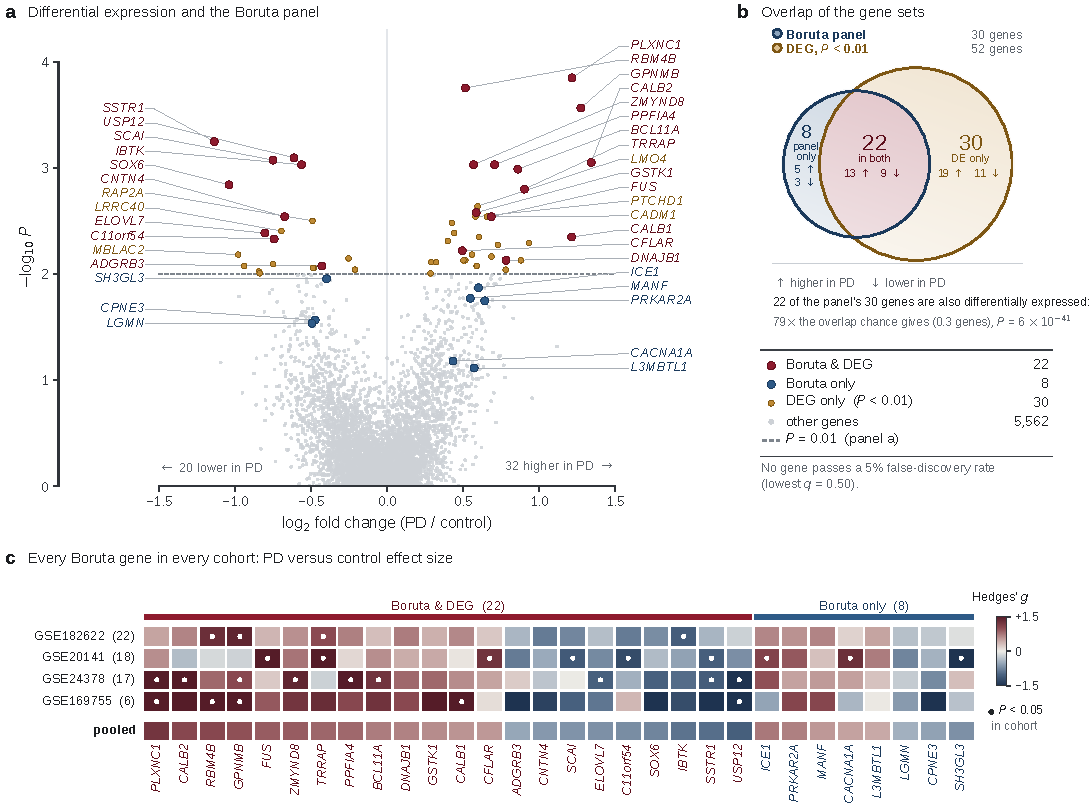
\includegraphics[width=\textwidth]{figures/Figure05_volcano_venn.pdf}
\caption{Differential expression and the panel. (a) Volcano of all 5,622 genes. (b) Overlap of the Boruta
panel with genes at $P<0.01$: 22 of 30, with the up and down split of each region; the overlap is 79 times
what chance gives. (c) Effect of every panel gene in every discovery cohort.}
\label{fig:volcano}
\end{figure}

\subsection{The frozen models in eight bulk cohorts}

Both models were fixed before the external data were touched. Applied without refitting to 158 donors in eight
bulk nigra cohorts, the core classifier pooled an AUC of 0.70 (95\% CI 0.62--0.78) and the panel forest 0.84
(0.77--0.90), both far from chance under within-cohort label permutation ($P<0.001$;
Fig.~\ref{fig:external}a, Table~\ref{tab:external}). At a cut-off fixed before testing the panel called 72\%
of donors correctly, with sensitivity 0.76 and specificity 0.68 (Fig.~\ref{fig:multicohort}b). Per-cohort AUCs
of the panel ranged from 0.43 in the 15-donor GSE20163 to 0.98 in GSE168496 (Fig.~\ref{fig:multicohort}a).
Retraining without any discovery study from the same brain bank changed little: 0.80 for the panel and 0.73
for the classifier. Dropping GSE7621, the cohort most similar to the discovery arrays, left the panel at 0.82.

\begin{figure}[htbp]\centering

\includegraphics[width=\textwidth]{figures/Figure06_external_validation.pdf}
\caption{External validation in eight bulk cohorts, 158 donors, both models frozen beforehand. (a) Weighted
average ROC of the classifier, the panel forest and a dopamine-neuron marker score. (b) Classifier score
against neuron content, with pooled AUCs after that content is removed. (c) Each panel gene's effect in
discovery and in bulk tissue, before and after the neuron adjustment.}
\label{fig:external}
\end{figure}

Chance is the wrong comparison here. Eight dopamine-neuron markers, averaged into a single score with no
model behind them, reached 0.86 in the same donors, better than either model. Removing that neuron
component from the scores within each cohort dropped the panel to 0.76 and the classifier to 0.62
(Table~\ref{tab:external}). Gene by gene is the test that matters for a panel offered as a set of candidates rather than
as a score. Twelve of the 30 genes reached $q<0.05$ in the bulk donors on their unadjusted effect, after
Benjamini--Hochberg correction over the panel, and nine of those twelve carried the same direction of effect as in the laser-captured
neurons: \textit{RBM4B}, \textit{USP12}, \textit{SOX6}, \textit{ADGRB3}, \textit{SH3GL3}, \textit{DNAJB1},
\textit{CNTN4}, \textit{ZMYND8} and \textit{SSTR1}. The other three, \textit{GSTK1}, \textit{PRKAR2A} and
\textit{CALB1}, were significant with the opposite sign, which is what a marker of the spared population looks
like once whole tissue rather than isolated neurons is measured. Across all 30, 19 effects had the same sign in bulk as in the laser-captured
neurons, which is not more than chance ($P=0.10$); after the neuron score is removed from every gene, 23 of 30
agree ($P=0.003$, Spearman $\rho=0.72$; Fig.~\ref{fig:external}c), and two genes, \textit{RBM4B} and
\textit{PLXNC1}, are still significant on their own at $q<0.05$ once that adjustment is made. Table~\ref{tab:genes}
reports the adjusted effect and its $q$ value for every gene, so the bulk row of that table is the conservative
version of the comparison made here. So the panel does say something about bulk nigra beyond counting neurons. Counting neurons still does the job
at least as well.

\begin{figure}[htbp]\centering
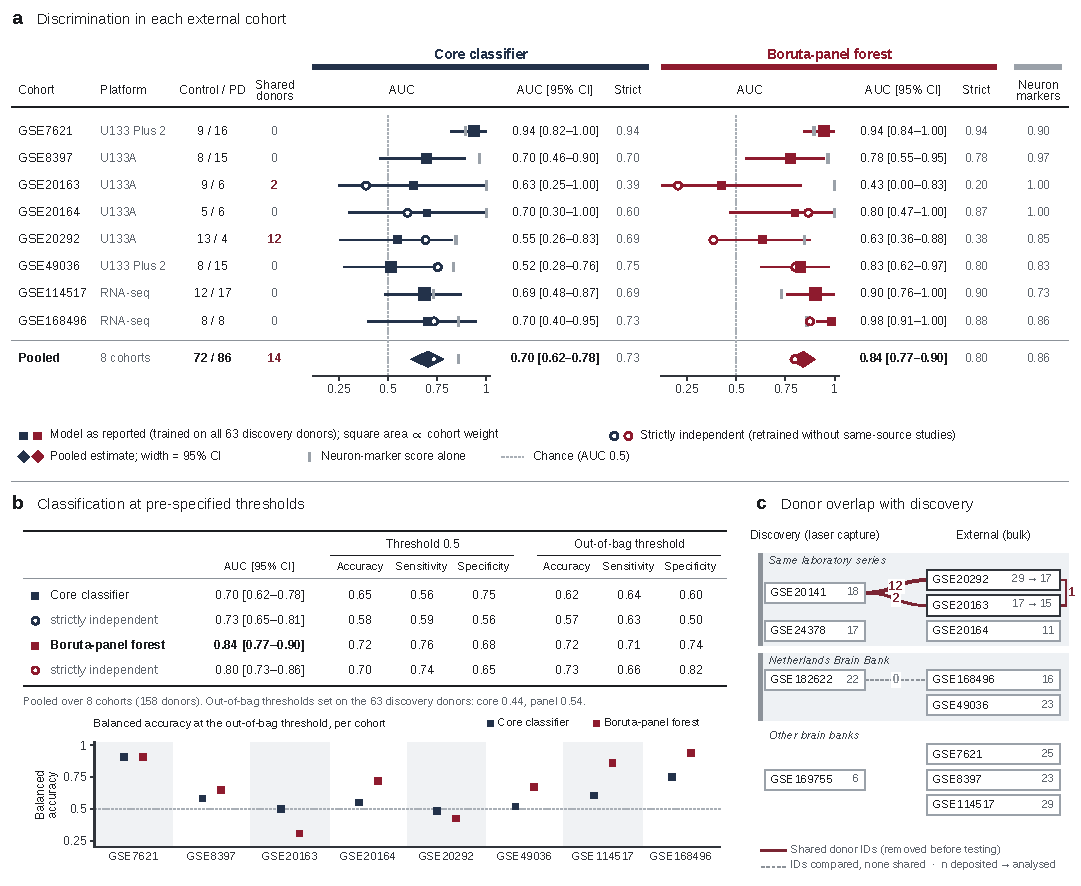
\includegraphics[width=\textwidth]{figures/Figure07_multicohort.pdf}
\caption{The frozen models cohort by cohort. (a) AUC of each cohort with bootstrap intervals and the pooled
estimate. (b) Calls at cut-offs fixed before testing. (c) Brains shared with the discovery studies, found by
donor identifier and removed.}
\label{fig:multicohort}
\end{figure}

\input{table_external}

Boruta reselected the panel genes at very different rates across the training folds, from \textit{RBM4B} in
every fold to \textit{MANF} and \textit{L3MBTL1} in four of twenty-five, so the panel was restricted by fold
frequency and retested. Keeping only the genes reselected in more than half of the folds leaves 14, and more
than 70\% leaves 8. Neither smaller panel does better. Pooled over the same donors the reported 30 genes
reach 0.772, the 14 stable genes 0.752 and the 8 most stable 0.725; every threshold between those points
lands in the same band. The tail of unstable genes is therefore contributing, not diluting, and the panel is
not improved by trimming it.

The comparison that decides how much of this is the panel rather than the method is 200 random panels of each
size, put through the identical procedure. All three panels beat their own null (
$P=0.015$, $0.015$ and $0.030$), but the null itself is high: a random 30-gene panel reaches a median pooled
AUC of 0.63, and one in twenty reaches 0.73. Any set of genes carries some of the neuron loss with it. The
selection adds to that, and the margin it adds is modest. These figures use all 173 external donors without
the donor-overlap removal, so they sit below the values in Table~\ref{tab:external} and are comparable with
each other rather than with that table.

\subsection{The panel tracks a dopamine-neuron lineage}

Three quarters of the panel genes appear in the Kamath single-nucleus marker table \citep{kamath2022}, and
they fall apart cleanly by direction. Genes lower in PD are markers of SOX6 dopamine neurons; genes higher are
markers of CALB1 neurons (difference in lineage score $P=0.0012$; each side also differs from the measured
background, $P=0.0066$ and $P=0.0038$; all two-sided Wilcoxon rank-sum tests; Fig.~\ref{fig:biology}). Because effect size and lineage could be
correlated through expression level, the same test was run against gene sets matched on differential
expression rank, and the split survived ($P=0.004$, one-sided by construction: the null is the
proportion of matched sets that separate at least as well). \textit{SOX6} itself is in the panel, lower in PD, as is
\textit{ADGRB3}; \textit{CALB1} and \textit{CALB2} are higher. This is the direction single-nucleus work
reports for selective vulnerability \citep{kamath2022}, recovered here from four bulk-processed LCM studies
that never saw a single-cell library.

\begin{figure}[htbp]\centering

\includegraphics[width=\textwidth]{figures/Figure08_panel_biology.pdf}
\caption{The panel against dopamine-neuron subtypes \citep{kamath2022}. (a) PD effect and lineage score of
every measured gene, with the panel marked. (b) Marker overlap by subtype. (c) Marker strength of each panel
gene in each subtype: genes lower in PD are SOX6 markers, genes higher are CALB1 markers.}
\label{fig:biology}
\end{figure}

\subsection{Pathways, with an honest background}

Using the 5,622 measured genes as the background and correcting across all 3,547 terms, the 30-gene panel
returns four significant terms: calcium ion binding involved in regulation of presynaptic cytosolic calcium
(FDR 0.005), excitatory synapse (0.016), a GO term labelled after cerebellar climbing-fibre synapses that
covers the same excitatory synaptic genes (0.018), and regulation of synapse pruning (0.028;
Fig.~\ref{fig:pathways}). Four terms is more than most random lists of the same size return: 32\% of random lists return at least one,
10\% return four or more, and the panel's strongest term beats 98\% of them. The enrichment is real and
modest. The terms rest on five genes: \textit{CALB1}, \textit{CALB2},
\textit{ADGRB3}, \textit{PLXNC1} and \textit{PPFIA4}. Four of those five are also lineage markers, so this is
close to the result of the previous section in different words.

\begin{figure}[htbp]\centering
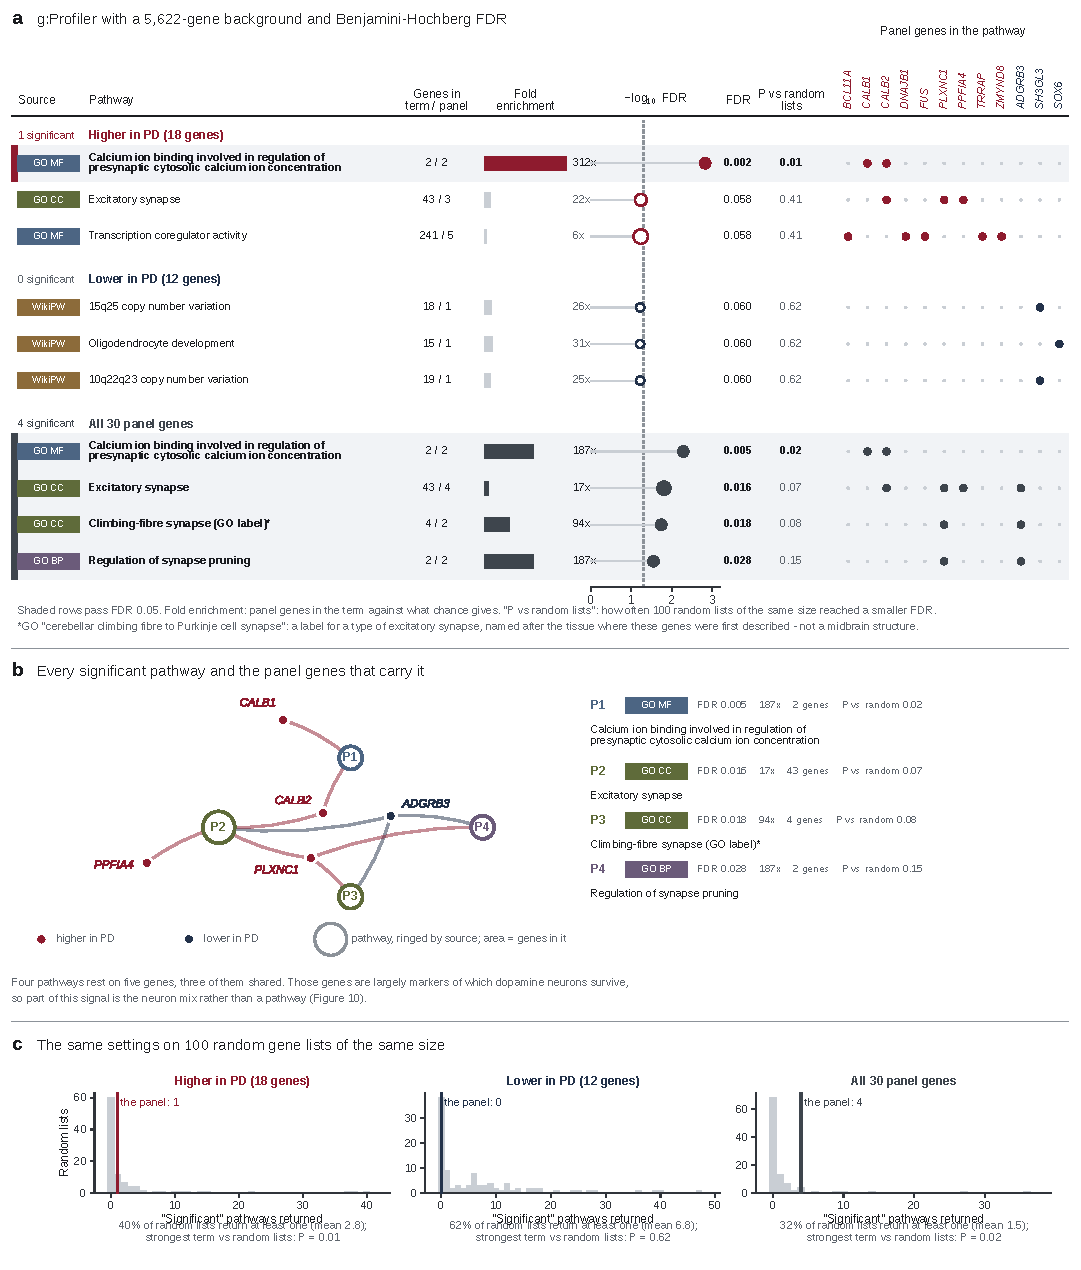
\includegraphics[width=\textwidth]{figures/Figure09_pathways.pdf}
\caption{Over-representation with the 5,622 measured genes as background and Benjamini-Hochberg correction.
(a) Terms for the lower, higher and full panel. (b) The four significant terms and the five genes that carry
them. (c) The same settings applied to 100 random gene lists of each size.}
\label{fig:pathways}
\end{figure}

A ranking-based analysis adds nothing that survives a strict null. Across 1,967 gene sets, none reaches
significance when the null is built by shuffling donor diagnoses within study; 20 pass the conventional
gene-permutation FDR of 0.25, of which 12 carry a panel gene in the leading edge, and single-sample scores
separate PD from control at $P<0.05$ for 147 sets but none after correction. We report those as exploratory,
not as findings \citep{subramanian2005}.

\subsection{How much of it is the neuron mix}

Each donor's dopamine-neuron subtype mix was estimated from the Kamath markers, with panel genes excluded.
PD donors are more CALB1-like than controls (AUC 0.73, Mann-Whitney $P=0.0003$), and the classifier's
out-of-fold score follows that mix ($\rho=0.51$ overall, 0.60 among controls alone), which is the correlation
one expects if the model is partly reading composition (Fig.~\ref{fig:mix}a,b).

Reference-based deconvolution says the same thing as the marker score, which is the point of running it.
Against the \citet{smajic2022} midbrain atlas, the estimated dopamine-neuron proportion tracks the
eight-marker score in every cohort (Spearman $\rho$ 0.57 to 0.99, all $P\le0.002$) and across the pooled
donors ($\rho=0.79$, $P=9\times10^{-39}$ for the variance-weighted estimator; 0.64 for $\nu$-SVR and 0.43 for
plain non-negative least squares, all $P<10^{-8}$). The deconvolution also recovers the disease itself
without being told about it: the dopamine-neuron fraction is the cell type that separates PD from control
most strongly and in the expected direction (median 6.2\% in controls against 0.0\% in PD, AUC 0.16, that is
0.84 for loss), while microglia, pericytes and oligodendrocyte precursors are higher in PD (AUC 0.65, 0.74
and 0.69). Residualising the external scores on the deconvolved proportion rather than on the marker score
costs the panel slightly more, not less: 0.77 to 0.67 against 0.77 to 0.73 on the same donors. The
composition explanation is therefore not an artefact of how we measured composition, and if anything the
marker score understates it.

Regressing the mix out of every gene and re-running the same folds with the same model is the test that
separates the two explanations. Out-of-fold AUC falls from 0.765 to 0.674, a drop that is well outside the fold-to-fold
variation, and the adjusted model still beats its own label permutations ($P=0.009$; Fig.~\ref{fig:mix}c).
Adding the classifier score to a model built on composition alone improves it (leave-one-out AUC 0.68 to 0.72,
likelihood-ratio $P=0.006$). Sensitivity runs with 25, 100 or 200 markers, with SOX6\_AGTR1 markers alone, or
with dopamine purity added, land between 0.64 and 0.76. Gene by gene, 23 of 30 keep at least half of their
effect, with a median of 68\% kept (Fig.~\ref{fig:mix}d, Table~\ref{tab:genes}).

So the signal is both things at once. A large part of what the classifier reads is which dopamine neurons
survive; a smaller part is a difference in the neurons that remain.

\begin{figure}[htbp]\centering
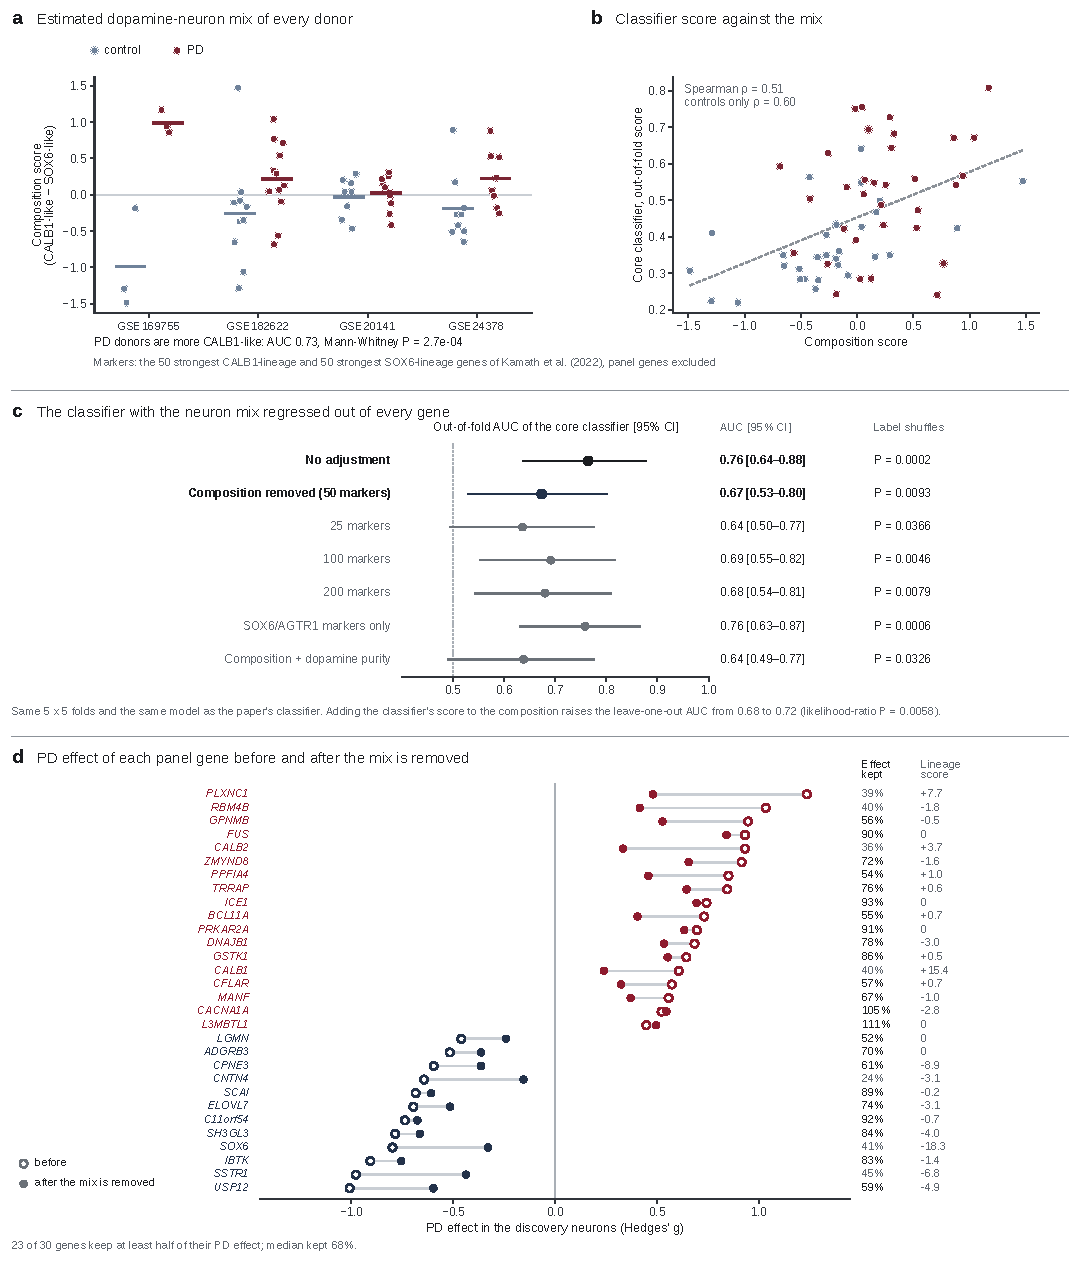
\includegraphics[width=\textwidth]{figures/Figure10_neuron_mix.pdf}
\caption{How much of the signal is the neuron mix. (a) Estimated CALB1-versus-SOX6 mix of every donor. (b) The
classifier's out-of-fold score against that mix. (c) Out-of-fold AUC with the mix regressed out of every gene,
across marker counts and variants. (d) Each panel gene's effect before and after the adjustment.}
\label{fig:mix}
\end{figure}

\subsection{The genes themselves}

Table~\ref{tab:genes} gives all 30 genes: the four measurements above, the dopamine-neuron subtype each one
marks, its Open Targets association with Parkinson disease, what is tractable about it, and any published
study tying it to the disease or to dopamine neurons.

Thirteen of the 30 carry such a study. Two of them, \textit{GPNMB} and \textit{ELOVL7}, sit at genetic risk
loci (Open Targets genetic association 0.78 and 0.51) \citep{buniello2025,blauwendraat2020}. \textit{SOX6}
and \textit{CALB1} are the markers of the vulnerable and the spared dopamine populations
\citep{kamath2022,damier1999}, and \textit{CALB2} is the third calcium-binding protein in that group: in
human PD midbrain its neurons were selectively preserved \citep{mouattprigent1994}. \textit{LGMN} encodes
legumain, which cleaves $\alpha$-synuclein at N103 and also truncates SOX6 in vulnerable neurons
\citep{zhang2017,nie2025}. \textit{DNAJB1} clears $\alpha$-synuclein through the Hsp70 system
\citep{huang2025}, \textit{MANF} restores nigrostriatal function after a 6-hydroxydopamine lesion
\citep{voutilainen2009}, and \textit{BCL11A} marks a nigral subset that is especially vulnerable to
$\alpha$-synuclein overexpression \citep{tolve2021}. That a wrapper algorithm with no knowledge of any of
this recovered thirteen such genes is the strongest evidence that the selection is not noise.

The other seventeen have no published tie to the disease, which is what makes them candidates rather than
confirmations. Which of them to follow depends on the composition adjustment rather than on the literature:
\textit{FUS} and \textit{DNAJB1} keep 90\% and 78\% of their effect once the neuron mix is removed, while
\textit{CNTN4} and \textit{CALB2} keep about a third, which is what a subtype marker looks like.

\section{Discussion}

A classifier trained on 63 laser-captured donors transfers to bulk nigra it has never seen: 0.70 for the
model, 0.84 for the 30-gene panel. The panel's directions match the SOX6--CALB1 split that single-nucleus
sequencing reports for selective vulnerability \citep{kamath2022}. When each donor's estimated subtype mix is
regressed out of every gene, the classifier loses about half of its margin over chance and keeps the rest.

The external result has to be read against the neuron-marker comparison. Eight markers with no model behind
them reach 0.86 in the same cohorts, above both trained models, and removing that component costs the panel
0.08 of AUC and the classifier 0.08 more. Composition explaining much of what looks like differential
expression is the rule in nigral tissue, not the exception \citep{nido2020}. The panel is not reducible to it:
after the neuron score is removed, 23 of 30 gene effects still agree in direction between laser-captured
neurons and bulk tissue ($P=0.003$), which a pure composition marker would not do. But any claim that a nigral
expression signature is diagnostic has to clear this bar first, and most published signatures have never been
asked to.

One number deserves more weight than its size suggests. Random 30-gene panels, selected without reference to
the disease and put through the same frozen procedure, reach a median pooled AUC of 0.63 in these cohorts,
and the best one in twenty reaches 0.73. A nigral expression panel therefore starts from a high floor,
because almost any gene set inherits some of the neuron loss. Read against that floor the panel is ahead but
not far ahead, and the honest description of the external result is a real effect of modest size rather than
a diagnostic. We report the null because a signature that has never been compared with a random one of equal
size has not been tested in the way that matters.

The two models do not transfer equally well, and the gap is informative. The panel forest reaches 0.84 in bulk
tissue while the core classifier reaches 0.70, although the core classifier is the better model in discovery.
The difference follows from what each one carries across. The core classifier's thirty components are fitted to
the total variance of 5,622 genes in laser-captured neurons, and a component is a weighted sum of all of them;
in bulk nigra the largest sources of variance are not the ones it was fitted on but platform, processing batch
and the ratio of glia to neurons, which behave differently in whole tissue than in a captured population
\citep{leek2010,nido2020}. A direction defined in one variance structure is only partly a direction in the
other, so the projection arrives distorted. The panel forest has no such projection: it reads thirty genes
that were each standardised within the receiving cohort, so a platform difference that shifts every gene
equally cancels, and only those thirty genes' behaviour is exposed. Narrow signatures transferring across
platforms better than dimension-reduced whole-transcriptome representations is the usual finding of
cross-study validation work \citep{bernau2014}, and it is the practical argument for reporting a gene list
rather than a fitted projection.

We did not expect the subtype result to hold. Boruta \citep{kursa2010} knows nothing about cell types, the
four studies predate the single-nucleus atlas, and the genes still sort by lineage at $P=0.0012$, and
$P=0.004$ against sets matched on effect size. That an unsupervised selection recovered an axis established
independently \citep{kamath2022,poulin2020} is reassuring about the method. It is also the least comfortable
finding here, because a panel that reports which dopamine neurons are left is measuring a consequence of the
disease rather than a mechanism inside the cells.

What survives the adjustment is a smaller signal, not an absent one. \textit{FUS}, \textit{DNAJB1},
\textit{TRRAP} and \textit{ZMYND8} keep the largest share of their effect, and they are chaperone, RNA-binding
and chromatin genes rather than subtype markers. \textit{DNAJB1} belongs to the HSP40 chaperone family, whose members differ in how well they
suppress seeded $\alpha$-synuclein aggregation \citep{deshayes2019}, and \textit{FUS} is an RNA-binding
protein central to work on RNA processing in neurodegeneration \citep{lagiertourenne2010}. Neither is a PD mechanism on this evidence. They are where we would look next, because their signal does not
dissolve when composition is removed.

Cause and consequence stay entangled here. All the tissue is post-mortem, and PD donors have already lost
most of the neurons the study is about \citep{kordower2013}.

The adjustment deserves more scepticism than it usually receives, including ours. Regressing a lineage score
out of every gene removes whatever part of that gene is linearly predictable from the score, and the score is
itself a contrast between CALB1 and SOX6 marker sets \citep{kamath2022}. Calcium buffering, synaptic vesicle
handling and the other processes most likely to fail in a stressed dopamine neuron are also the processes
that distinguish those two populations in the first place \citep{surmeier2017,poulin2020}. A gene whose
disease response runs along that axis is therefore partly removed as composition even when the change is
real and intrinsic, and no amount of care in fitting the regression can separate two effects that are
collinear in the data at hand. The adjusted figure of 0.67 is best read as a lower bound on what survives
inside surviving neurons, and the unadjusted 0.76 as an upper bound.

Two further limits of the procedure point in opposite directions, which is why we report the bracket rather
than a point estimate. The regression is linear and assumes the composition effect is additive on the z scale;
a non-linear relation would leave residual composition behind. Against that, the covariate is estimated with
error rather than measured, and regression on a covariate that carries measurement error is attenuated, so
the correction applied is smaller than the one intended \citep{frost2000}. Three observations argue that the adjustment has not simply erased the
biology: 23 of 30 genes keep at least half of their effect, agreement of sign between laser-captured neurons
and bulk tissue \emph{rises} after the adjustment rather than falling (19 of 30 to 23 of 30, $P=0.003$), and
an independent deconvolution against a single-nucleus atlas reaches the same composition estimate
\citep{smajic2022,newman2015,wang2019}. The sensitivity runs point the same way: the result holds between 25
and 200 markers, with SOX6\_AGTR1 markers alone, and with dopamine purity added. What would settle the
question is not a better regression but better measurement, that is subtype proportions counted directly in
the same donors, by single-nucleus or spatial profiling, rather than inferred from bulk expression.

\subsection*{Limitations}

The discovery cohort is 63 people, which is large for laser-capture nigra and small for machine learning; no
gene passes a genome-wide false-discovery threshold, and the panel should be read as a stable selection, not a
list of established PD genes. The external cohorts are bulk tissue, so the transfer is across both study and
tissue type, and cohort sizes run from 11 to 29 donors, which makes individual cohort AUCs unstable. Boruta selection is itself
unstable at this sample size: rerun on the donors that remain after a whole brain bank is withheld, it returns
panels sharing 5 of 30 and 15 of 32 genes with the reported one, so the panel is one of several
near-equivalent all-relevant sets that these data support, and the nine genes that replicate externally carry
more weight than membership of the list. Restricting the panel to its stable core does not repair this:
the 14 genes reselected in more than half of the folds, and the 8 reselected in more than 70\%, transfer
slightly worse than the full 30, so the instability cannot be removed by trimming. Donor overlap could only be excluded where identifiers allowed it; the strictly independent models are the guard
against what identifiers missed. Subtype mixtures are estimated from marker averages, not measured, and the
Kamath markers come from a different cohort and technology \citep{kamath2022}. Finally, clinical detail is
thin in the public metadata: we could not test disease duration, medication or Braak stage systematically,
though the early-stage cohort GSE49036 \citep{dijkstra2015} scored no differently from the rest.

\subsection*{Data and code availability}

Every dataset used here is public in the Gene Expression Omnibus \citep{barrett2013}. The discovery
cohort is four laser-capture studies of nigral dopamine neurons: GSE182622 \citep{tiklova2021}, GSE20141
and GSE24378 \citep{zheng2010}, and GSE169755 \citep{zaccaria2022}. The models were then tested in eight
bulk substantia nigra cohorts: GSE7621 \citep{lesnick2007}, GSE8397 \citep{moran2006}, GSE20163 and
GSE20164 \citep{zheng2010}, GSE20292 \citep{zhang2005}, GSE49036 \citep{dijkstra2015}, GSE114517
\citep{simchovitz2020} and GSE168496 \citep{tranchevent2023}. Dopamine-neuron subtype markers are
Supplementary Table 8 of \citet{kamath2022}. Gene annotation came from UniProt \citep{uniprot2025}, target
information from the Open Targets Platform \citep{buniello2025}, and the literature search from Europe PMC
\citep{europepmc2024}.

All code is public at \url{https://github.com/Alisareminia/pd-lcm-boruta}: the seventeen notebooks as they
were run, the scripts that generate them, the tables behind every figure, and the figures themselves. Each
notebook reads the outputs of the ones before it, so any figure can be redrawn without repeating the
analysis. The record of the literature search, with every hit and whether it was kept, is Supplementary
Table~S1.

\printbibliography[title={References}]

\clearpage

\input{table3_genes}

\end{document}
